\begin{fact}
	$\forall x \in \RR$,
	$\sder{\exp}{1} x = \exp x$.
\end{fact}


\begin{proof}
	Notons $\setproba{L}$ et $\setproba{E}$ les représentations graphiques respectives des fonctions $\ln$ et $\exp$.
	%
	Nous savons que $\setproba{L}$ et $\setproba{E}$ sont symétriques par rapport à la droite $\Delta: y = x$.
	Pour $h \neq 0$, considérons 
	$A(a ; \exp a) \in \setproba{E}$ et $M(a+h ; \exp(a+h)) \in \setproba{E}$.
	Par symétrie, nous avons
	$B(\exp a ; a) \in \setproba{L}$ et $N(\exp(a+h) ; a+h) \in \setproba{L}$.
	
	Examinons si le taux d'accroissement $\frac{\exp(a+h) - \exp a}{h}$ admet une limite en $0$.
	Ce quotient est la pente $m(AM)$ de la droite $(AM)$,
	or $m(AM) = \frac{1}{m(BN)}$.
	%
	En raisonnant sur $\setproba{L}$, faire tendre $h$ vers $0$ n'est possible que si $x(N)$ tend vers $x(B)$.
	Comme $\ln$ est dérivable en $x(B)$, nous obtenons $\limit{(m(BN))}{h}{0} = \der{\ln}{x}{1}(x(B)) = \frac{1}{\exp a}$.
	%
	Finalement,
	$\limit{(\frac{\exp(a+h) - \exp a}{h})}{h}{0} = \exp a$
	comme souhaité.

	\begin{center}
		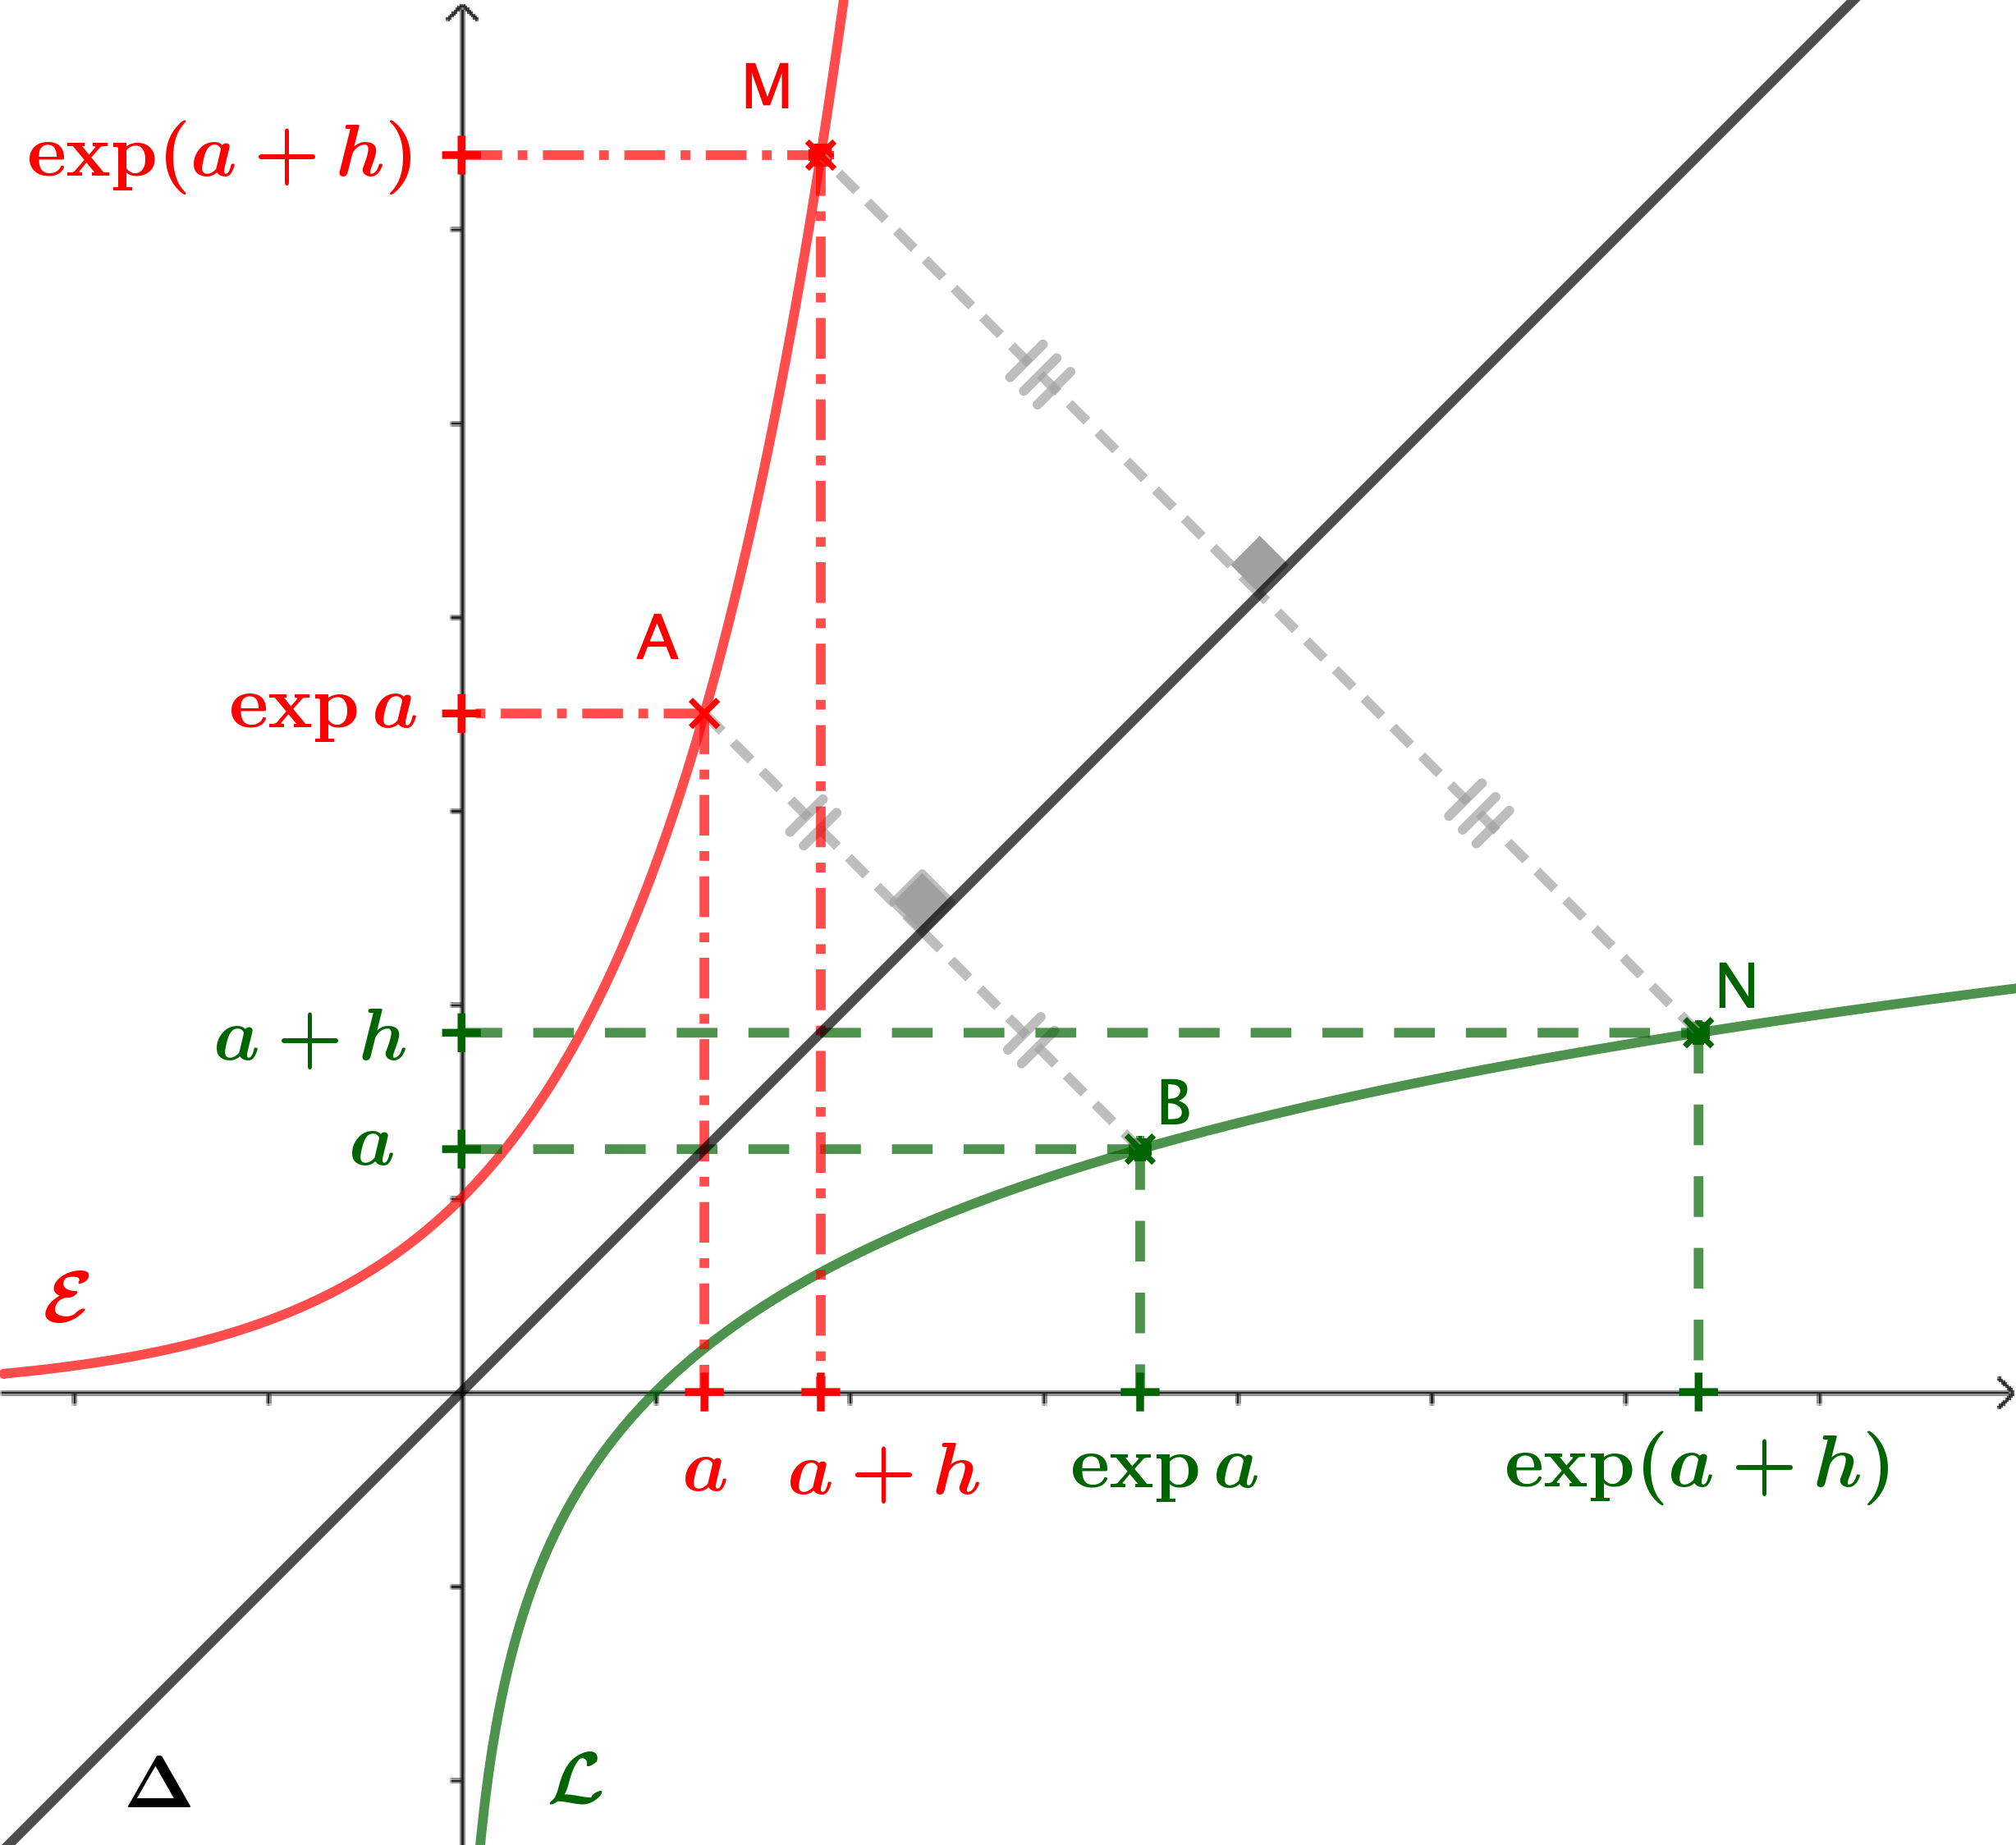
\includegraphics[scale=.85]{content/exp/eq-diff.png}
	\end{center}
\end{proof}